
\section{Avaliação}
	\label{sec:avaliacao}


%avaliação
%todos precisam de um gold text
%
%	1 - Concatenação
%	2 - Juízes concordam ou não 
%	3 - Mediador na reunião
%	4 - Não avaliar o segmentador e sim o resultado da aplicação final.
%	5 - Consultar o autor do texto

Para que se possa avaliar um segmentador automático de textos, é preciso uma referência, isto é, um texto com os limites entre os segmento conhecidos. Essa referência, deve ser confiável, sendo uma segmentação legítima que é capaz de dividir o texto em porções relativamente independentes, mantendo um conteúdo legível, ou seja, uma segmentação ideal.
%

Entre as abordagens mais comuns para se conseguir essas referências, encontramos: A concatenação aleatória de documentos distintos, onde o ponto entre o final de um texto e o inicio do seguinte é um limite entre eles. A segmentação manual dos documentos, nesse caso, pessoas capacitadas, também chamadas de juízes, ou mesmo o autor do texto, são consultadas e indicam manualmente onde há uma quebra de segmento. Em transcrição de conversas faladas em reuniões com múltiplos participantes, um mediador é responsável por encerrar um assunto e iniciar um novo, nesse caso o mediador anota manualmente o tempo onde há uma transição de tópico. Em aplicações onde a segmentação é tarefa secundária, analisar seu impacto na aplicação final.


% Definir o que é um bom algoritmo de segmentação

Para fins de avaliação, um bom método de segmentação


	
	

De acordo com \cite{fulano} há duas principais dificuldades na avaliação de segmentadores automáticos. A primeira é conseguir um referência, já que juízes humanos costumam não concordar entre si, sobre onde os limites estão e outras abordagens podem não se aplicar ao contexto. A segunda é que tipos diferentes de erros devem ter pesos diferentes de acordo com a aplicação. Há casos onde certa imprecisão é tolerável e outras como a segmentação de notícias, onde a precisão é mais importante.

%Para contornar essas dificuldades, algumas abordagens podem ser utilizadas. Algumas autores preferem detectar a segmentação em textos formados pela concatenação de documentos distintos, para que não haja diferenças subjetivas \cite{Reynar 1994; Choi 2000; e própiro autor do "A Critique and Impro.}. Há ainda outros que não avaliam o algoritmo diretamente, mas seu impacto na aplicação final\cite{Manning 1998; Kan,
%Klavans, and McKeown 1998}. 
%Outras abordagens apenas atribuiem um segmento cada quebra de parágrafo \cite{Two Step ... Meeting Minutes}


% Dificuldade: Coesão léxica não tão bem definida
O vocabulário das reuniões, ainda que em tópicos diferentes, compartilham certo vocabulário pertencente ao ambiente onde as se deram as reuniões. Isso é um fator que diminui a o princípio da coesão léxica entre os segmentos.


\subsection{Medidas de Avaliação}


	As medidas de avaliação tradicionalmente utilizadas em \textit{information retrieval} como precisão e revocação trazem alguns problemas na avalização de segmentadores automáticos.  
Conforme o algoritmo aponta mais segmentos no texto, tende a melhorar a revocação e ao mesmo tempo, reduzir a precisão, um problema que pode ser contornado usando F1 que faz uma combinação da duas levando em conta seus pesos, o que por outro lado é mais difícil de interpretar. 
Essas medidas falham ao não serem sensíveis a \textit{near misses}, ou seja, quando um limite não coincide exatamente com o esperado, mas fica próximo~\cite{Kern2009167}.

A Figura~\ref{fig:exemplosegmentacaozoom} mostra um exemplo com duas segmentações hipotéticas e uma referência. Em ambos os casos não há nenhum verdadeiro positivo, o que implica em zero para os valores de precisão, acurácia, e revocação, embora a segunda hipótese possa ser considerada superior à primeira se levado em conta a proximidade dos limites.



  \begin{figure}[!h]

	\centering
	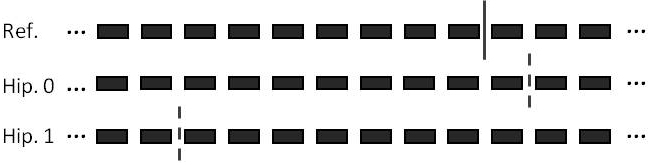
\includegraphics[width=0.47\textwidth]{windiffzoom.jpg}
	\caption{Exmplos de segmentação}
	\label{fig:exemplosegmentacaozoom}

  \end{figure}



\subsubsection{P$_k$}
A fim de resolver o problema de \textit{near misses}, Beeferman \textit{at al.}~\cite{Beeferman1999} apresentam uma nova medida chama P$_k$ que atribui valores parciais a \textit{near misses}. Esse método move uma janela de tamanho $k$ e a cada posição e verifica se o início e o final da janela estão ou não dentro do mesmo segmento e penaliza o algoritmo em caso de discrepância. 

Ou seja, dado duas palavras de distancia $k$, uma discrepância é computada quando o algoritmo e a referência não concordam se as palavras estão ou não no mesmo segmento.

O valor de $k$ é calculado como a metade da média dos comprimentos dos segmentos reais. Como resultado, é retornado a contagem de discrepâncias divido pelo quantidade de segmentações analisadas. Esse valor serve como medida de dissimilaridade entre as segmentações e pode ser interpretada como a probabilidade de duas sentenças extraídas aleatoriamente pertencerem ao mesmo segmento.



\subsubsection{WindowDiff}

Pevzner~\cite{Pevzner200219} aponta problemas na avaliação mais tradicional Pk~\cite{Beeferman1999}. Eles apontam que esse método penaliza demasiadamente os falsos negativos em relação aos falsos positivos e a \textit{near misses}, além disso, desconsidera o tamanho e a quantidade de segmentos, entre outros problemas.

Como solução, propõem um novo método, o qual chamam de \textit{WindowDiff} que traz duas diferenças principais: a dobra a penalidade para os falsos positivos a fim de diminuir o problema da subestimação dessa medida e, diferente de P$_k$, ao mover a janela pelo texto, penaliza o algoritmo sempre que o número de limites proposto pelo algoritmo não coincidir com o número de limites esperados para aquela janela de texto. 

Com isso, demonstram em seu trabalho que, em relação a P$_k$, consegue resolver seus principais problemas e mantém sua proposta inicial de sensibilidade a \textit{near misses}, penalizando-os menos que os falsos positivos puros.


  \begin{figure}[!h]

	\centering
	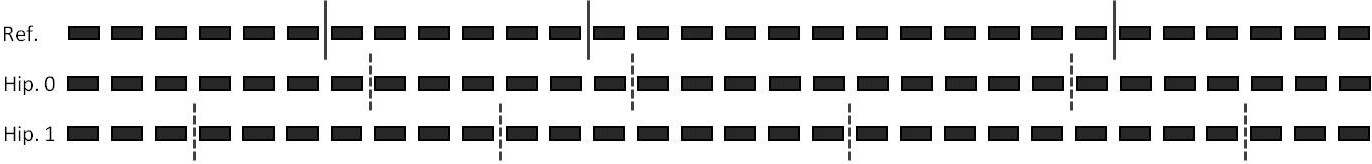
\includegraphics[width=0.47\textwidth]{windiff.jpg}
	\caption{Exemplo de construção de uma matriz de rank}
	\label{fig:exemplosegmentacao}

  \end{figure}
  
  

%Falar do software para segmentação manual????

